\documentclass[]{article}
\usepackage{lmodern}
\usepackage{amssymb,amsmath}
\usepackage{ifxetex,ifluatex}
\usepackage{fixltx2e} % provides \textsubscript
\ifnum 0\ifxetex 1\fi\ifluatex 1\fi=0 % if pdftex
  \usepackage[T1]{fontenc}
  \usepackage[utf8]{inputenc}
\else % if luatex or xelatex
  \ifxetex
    \usepackage{mathspec}
  \else
    \usepackage{fontspec}
  \fi
  \defaultfontfeatures{Ligatures=TeX,Scale=MatchLowercase}
\fi
% use upquote if available, for straight quotes in verbatim environments
\IfFileExists{upquote.sty}{\usepackage{upquote}}{}
% use microtype if available
\IfFileExists{microtype.sty}{%
\usepackage{microtype}
\UseMicrotypeSet[protrusion]{basicmath} % disable protrusion for tt fonts
}{}
\usepackage[margin=1in]{geometry}
\usepackage{hyperref}
\hypersetup{unicode=true,
            pdftitle={Introduction to R},
            pdfborder={0 0 0},
            breaklinks=true}
\urlstyle{same}  % don't use monospace font for urls
\usepackage{color}
\usepackage{fancyvrb}
\newcommand{\VerbBar}{|}
\newcommand{\VERB}{\Verb[commandchars=\\\{\}]}
\DefineVerbatimEnvironment{Highlighting}{Verbatim}{commandchars=\\\{\}}
% Add ',fontsize=\small' for more characters per line
\usepackage{framed}
\definecolor{shadecolor}{RGB}{248,248,248}
\newenvironment{Shaded}{\begin{snugshade}}{\end{snugshade}}
\newcommand{\AlertTok}[1]{\textcolor[rgb]{0.94,0.16,0.16}{#1}}
\newcommand{\AnnotationTok}[1]{\textcolor[rgb]{0.56,0.35,0.01}{\textbf{\textit{#1}}}}
\newcommand{\AttributeTok}[1]{\textcolor[rgb]{0.77,0.63,0.00}{#1}}
\newcommand{\BaseNTok}[1]{\textcolor[rgb]{0.00,0.00,0.81}{#1}}
\newcommand{\BuiltInTok}[1]{#1}
\newcommand{\CharTok}[1]{\textcolor[rgb]{0.31,0.60,0.02}{#1}}
\newcommand{\CommentTok}[1]{\textcolor[rgb]{0.56,0.35,0.01}{\textit{#1}}}
\newcommand{\CommentVarTok}[1]{\textcolor[rgb]{0.56,0.35,0.01}{\textbf{\textit{#1}}}}
\newcommand{\ConstantTok}[1]{\textcolor[rgb]{0.00,0.00,0.00}{#1}}
\newcommand{\ControlFlowTok}[1]{\textcolor[rgb]{0.13,0.29,0.53}{\textbf{#1}}}
\newcommand{\DataTypeTok}[1]{\textcolor[rgb]{0.13,0.29,0.53}{#1}}
\newcommand{\DecValTok}[1]{\textcolor[rgb]{0.00,0.00,0.81}{#1}}
\newcommand{\DocumentationTok}[1]{\textcolor[rgb]{0.56,0.35,0.01}{\textbf{\textit{#1}}}}
\newcommand{\ErrorTok}[1]{\textcolor[rgb]{0.64,0.00,0.00}{\textbf{#1}}}
\newcommand{\ExtensionTok}[1]{#1}
\newcommand{\FloatTok}[1]{\textcolor[rgb]{0.00,0.00,0.81}{#1}}
\newcommand{\FunctionTok}[1]{\textcolor[rgb]{0.00,0.00,0.00}{#1}}
\newcommand{\ImportTok}[1]{#1}
\newcommand{\InformationTok}[1]{\textcolor[rgb]{0.56,0.35,0.01}{\textbf{\textit{#1}}}}
\newcommand{\KeywordTok}[1]{\textcolor[rgb]{0.13,0.29,0.53}{\textbf{#1}}}
\newcommand{\NormalTok}[1]{#1}
\newcommand{\OperatorTok}[1]{\textcolor[rgb]{0.81,0.36,0.00}{\textbf{#1}}}
\newcommand{\OtherTok}[1]{\textcolor[rgb]{0.56,0.35,0.01}{#1}}
\newcommand{\PreprocessorTok}[1]{\textcolor[rgb]{0.56,0.35,0.01}{\textit{#1}}}
\newcommand{\RegionMarkerTok}[1]{#1}
\newcommand{\SpecialCharTok}[1]{\textcolor[rgb]{0.00,0.00,0.00}{#1}}
\newcommand{\SpecialStringTok}[1]{\textcolor[rgb]{0.31,0.60,0.02}{#1}}
\newcommand{\StringTok}[1]{\textcolor[rgb]{0.31,0.60,0.02}{#1}}
\newcommand{\VariableTok}[1]{\textcolor[rgb]{0.00,0.00,0.00}{#1}}
\newcommand{\VerbatimStringTok}[1]{\textcolor[rgb]{0.31,0.60,0.02}{#1}}
\newcommand{\WarningTok}[1]{\textcolor[rgb]{0.56,0.35,0.01}{\textbf{\textit{#1}}}}
\usepackage{graphicx,grffile}
\makeatletter
\def\maxwidth{\ifdim\Gin@nat@width>\linewidth\linewidth\else\Gin@nat@width\fi}
\def\maxheight{\ifdim\Gin@nat@height>\textheight\textheight\else\Gin@nat@height\fi}
\makeatother
% Scale images if necessary, so that they will not overflow the page
% margins by default, and it is still possible to overwrite the defaults
% using explicit options in \includegraphics[width, height, ...]{}
\setkeys{Gin}{width=\maxwidth,height=\maxheight,keepaspectratio}
\IfFileExists{parskip.sty}{%
\usepackage{parskip}
}{% else
\setlength{\parindent}{0pt}
\setlength{\parskip}{6pt plus 2pt minus 1pt}
}
\setlength{\emergencystretch}{3em}  % prevent overfull lines
\providecommand{\tightlist}{%
  \setlength{\itemsep}{0pt}\setlength{\parskip}{0pt}}
\setcounter{secnumdepth}{0}
% Redefines (sub)paragraphs to behave more like sections
\ifx\paragraph\undefined\else
\let\oldparagraph\paragraph
\renewcommand{\paragraph}[1]{\oldparagraph{#1}\mbox{}}
\fi
\ifx\subparagraph\undefined\else
\let\oldsubparagraph\subparagraph
\renewcommand{\subparagraph}[1]{\oldsubparagraph{#1}\mbox{}}
\fi

%%% Use protect on footnotes to avoid problems with footnotes in titles
\let\rmarkdownfootnote\footnote%
\def\footnote{\protect\rmarkdownfootnote}

%%% Change title format to be more compact
\usepackage{titling}

% Create subtitle command for use in maketitle
\providecommand{\subtitle}[1]{
  \posttitle{
    \begin{center}\large#1\end{center}
    }
}

\setlength{\droptitle}{-2em}

  \title{Introduction to R}
    \pretitle{\vspace{\droptitle}\centering\huge}
  \posttitle{\par}
    \author{}
    \preauthor{}\postauthor{}
    \date{}
    \predate{}\postdate{}
  

\begin{document}
\maketitle

\hypertarget{introduction-to-r}{%
\subsection{Introduction to R}\label{introduction-to-r}}

Contents borrowed and modified from
\href{https://uvastatlab.github.io/phdplus/intror.html}{UVA's Data
Science Essentials in R series} and RStudio's
\href{https://github.com/rstudio-education/master-the-tidyverse/blob/master/slides/00-Introduction.pdf}{Master
the Tidyverse} workshop.

\hypertarget{installation}{%
\subsubsection{Installation}\label{installation}}

Instructions for how to install and/or update R, RStudio, and the
\texttt{tidyverse} package can be found
\href{preworkshop_instructions.html}{here}.

\hypertarget{features-of-r}{%
\subsubsection{Features of R}\label{features-of-r}}

\begin{itemize}
\tightlist
\item
  R is free!
\item
  R is everywhere, and has an active user base. This is useful because
  you can find a lot of people in various disciplines using R in blogs,
  forums, Stack Overflow, etc., and you can often find help online
  there.
\item
  R is flexible! Since R is open source, the active R user base
  implements new methods as libraries in R quickly. Over 10,000 packages
  are available.
\item
  R is cool! It is highly regarded for its:

  \begin{itemize}
  \tightlist
  \item
    Graphical functionality. See
    \href{https://ggplot2.tidyverse.org/}{gplot2},\href{http://www.ggplot2-exts.org/gallery/}{ggplot
    extensions}.
  \item
    Interactive web functionality. See
    \href{https://shiny.rstudio.com/gallery/}{shiny}.
  \item
    Reproducible output, such as documents, presentations, and
    dashboards. See
    \href{https://rmarkdown.rstudio.com/gallery.html}{markdown}.
  \item
    Easy integration with other open-source or data science
    applications, such as Sublime Text, Jupyter Notebooks, GitHub, etc.
  \end{itemize}
\end{itemize}

\begin{center}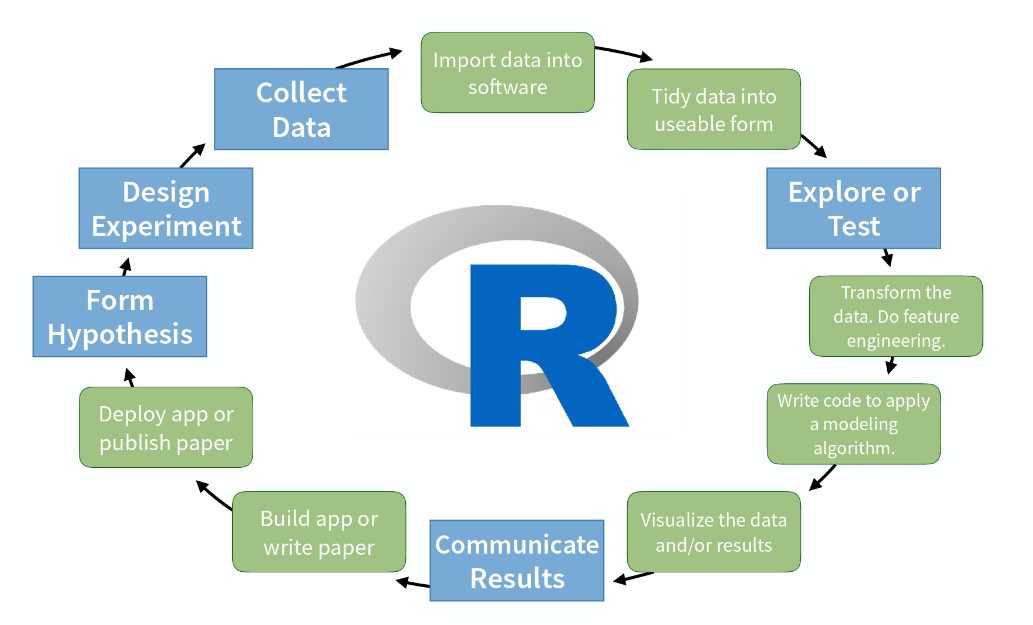
\includegraphics[width=0.9\linewidth]{images/data-science-R} \end{center}

\hypertarget{orientation-to-r-and-rstudio}{%
\subsection{Orientation to R and
RStudio}\label{orientation-to-r-and-rstudio}}

We recommend that you use R with RStudio. R is the base statistical
computing environment. RStudio is an ``Interactive Development
Environment'' makes it easy to use R. It does things like auto-complete,
syntax highlighting, and is generally much easier to use. After you
install R and RStudio, you only need to run RStudio. RStudio shows four
panes by default. The two most important are the Console (bottom left)
and the Script Editor (top left).

This is what RStudio looks like when you first open it:

\begin{center}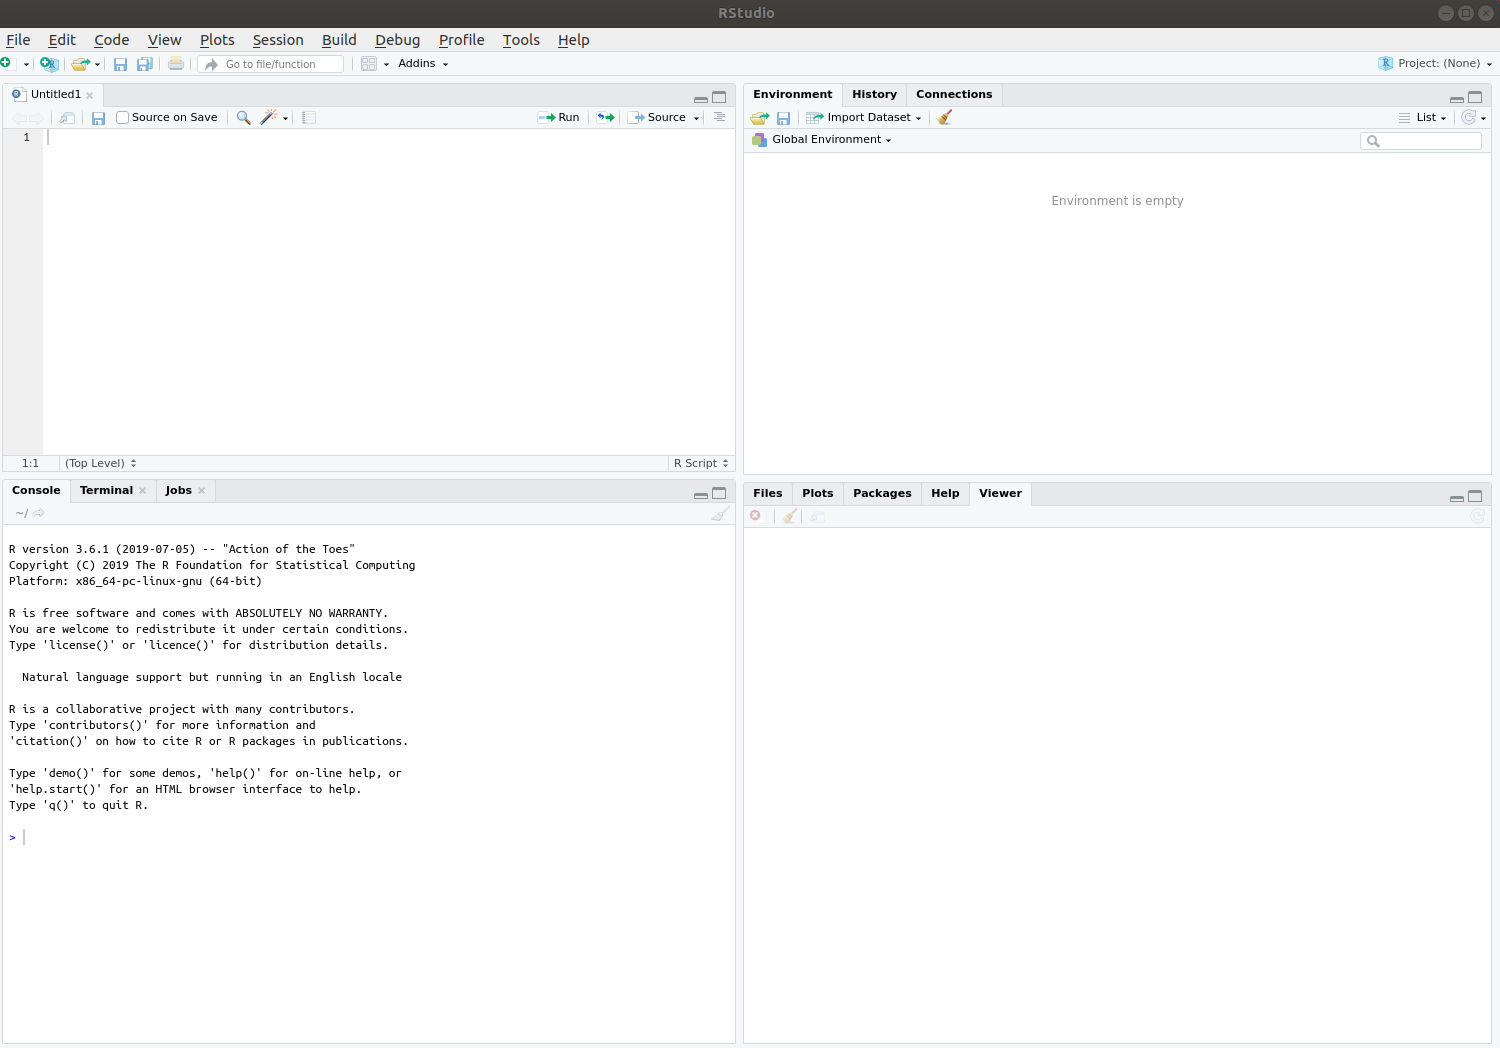
\includegraphics[width=0.9\linewidth]{images/RStudio} \end{center}

\hypertarget{console-bottom-left}{%
\subsubsection{Console (bottom left)}\label{console-bottom-left}}

The console pane allows you to quickly and immediately execute R code.
You can experiment with functions here, or quickly print data for
viewing. Type next to the \textgreater{} and press Enter to execute.

\begin{center}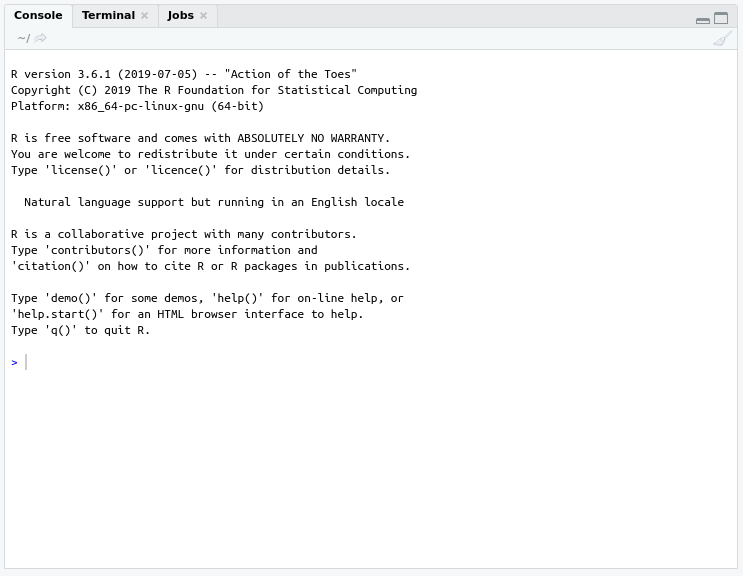
\includegraphics[width=0.9\linewidth]{images/console} \end{center}

\textbf{Console Practice}

You can use R like a calculator. Try typing 2+5 into the console.

\begin{Shaded}
\begin{Highlighting}[]
\DecValTok{2}\OperatorTok{+}\DecValTok{8}
\CommentTok{#> [1] 10}
\end{Highlighting}
\end{Shaded}

Here, the plus sign is the \textbf{operator}. Operators are symbols that
represent some sort of action. Of course, it would be silly if we only
used R as a calculator. To use R more fully, we need to understand
\textbf{objects}, \textbf{functions}, and \textbf{indexing} - which we
will learn about as we go.

For now, think of \emph{objects as nouns} and \emph{functions as verbs}.

\hypertarget{script-editor-top-left}{%
\subsubsection{Script Editor (top left)}\label{script-editor-top-left}}

In contrast to the Console, which quickly runs code, the Script Editor
does not automatically execute code. The Script Editor allows you to
save the code essential to your analysis. You can re-use that code in
the moment, refer back to it later, or publish it for replication. When
writing scripts do your future self a favor and use lots of comments!
Preface comments with a hashtag: `\#'. Good to know: R script files end
with ``.R''

\begin{center}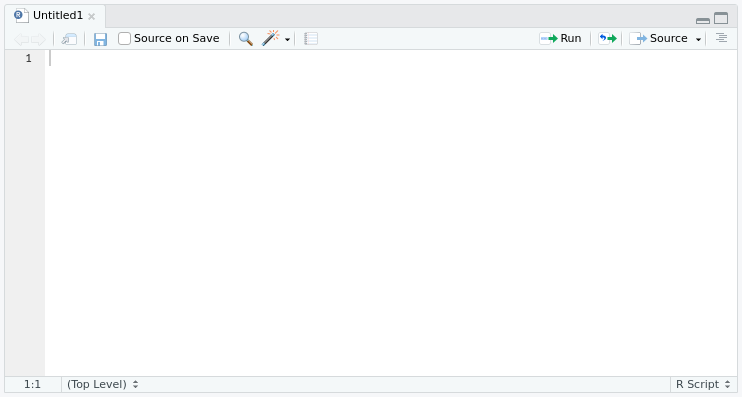
\includegraphics[width=0.9\linewidth]{images/script-editor} \end{center}

\textbf{Running commands from a script}

To run code from a script, insert your cursor on a line with a command,
and press CTRL+Enter/CMD+Enter.

Or highlight some code to only run certain sections of the command, then
press CTRL+Enter/CMD+Enter to run.

Alternatively, use the Run button at the top of the pane to execute the
current line or selection.

\hypertarget{other-panes}{%
\subsubsection{Other Panes}\label{other-panes}}

\begin{center}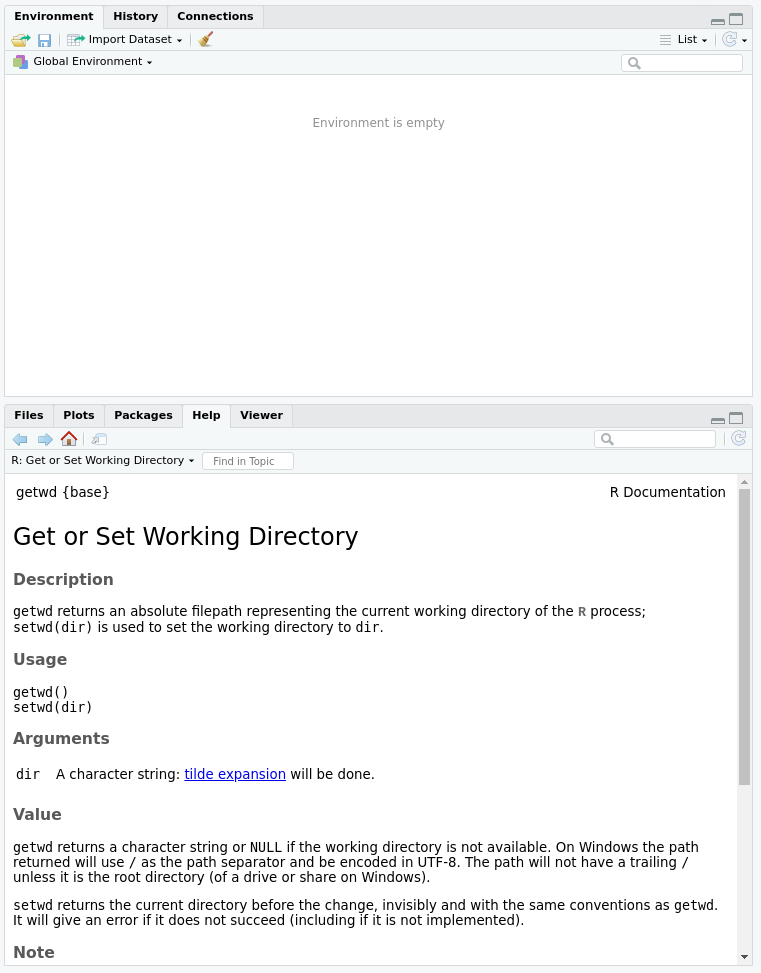
\includegraphics[width=0.9\linewidth]{images/other-panes} \end{center}

The other panes are on the right of the screen.

\begin{itemize}
\tightlist
\item
  \textbf{Environment} (top): Lists all currently defined objects and
  data sets.
\item
  \textbf{History} (top): Lists all commands recently used or associated
  with a project.
\item
  \textbf{Connections} (top): Lists connections to data sources
  (e.g.~Spark).
\item
  \textbf{Files} (bottom): Shows the files available to you in your
  working directory.
\item
  \textbf{Plots} (bottom): Graphical output goes here.
\item
  \textbf{Packages} (bottom): Lists all installed packages. Packages
  with checks next to them are currently loaded.
\item
  \textbf{Help} (bottom): Find help for R packages and functions. Don't
  forget you can type ? before a function name in the console to get
  info in the Help section.
\item
  \textbf{Viewer} (bottom): Renders HTML documents (created with
  RMarkdown).
\end{itemize}

\hypertarget{using-packages}{%
\subsection{Using Packages}\label{using-packages}}

Packages contain functions, and all functions belong to packages. R
comes with about 30 packages (``base R''). There are over 10,000
user-contributed packages; you can discover these packages online. A
prevalent collection of packages is the Tidyverse, which includes
\texttt{ggplot2}, a package for making graphics.

\begin{center}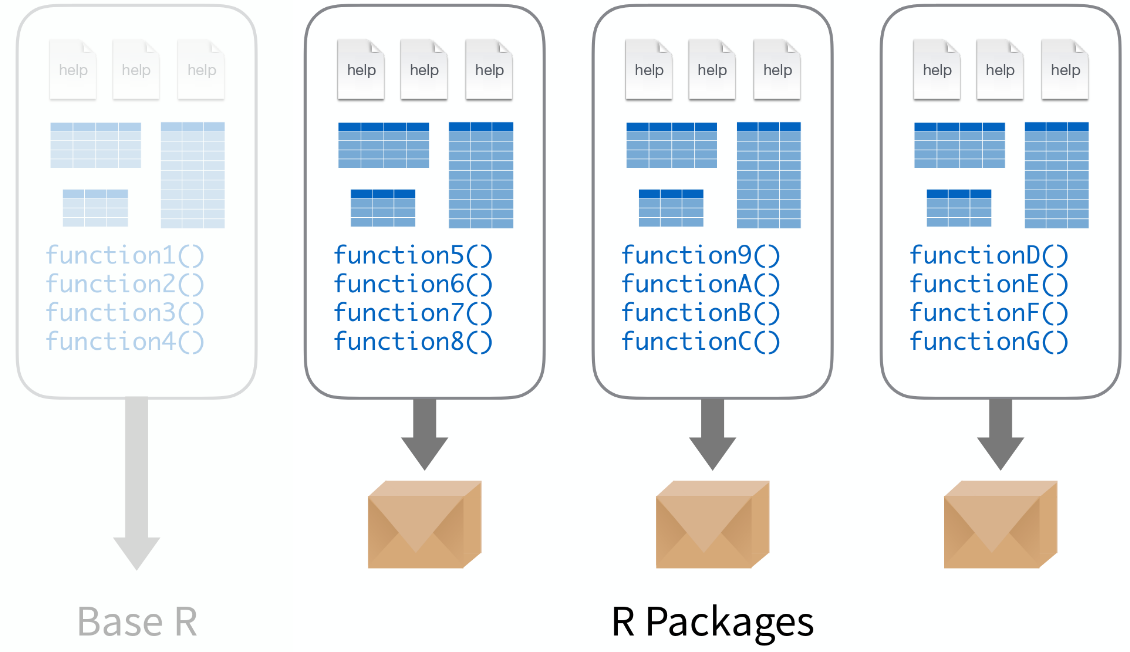
\includegraphics[width=0.9\linewidth]{images/packages} \end{center}

Only install a package once. It will likely install several other
packages it depends on. You should have already installed
\texttt{tidyverse} before the workshop.

You can install packages via point-and-click:
\texttt{Tools}--\textgreater{} \texttt{Install\ Packages}. Enter
\texttt{tidyverse} (or a different package name) then click
\texttt{Install}.

Or you can use this command in the console:
\texttt{install.packages("tidyverse")}

You must load the package in any new R session where you want to use
that package. Loading \texttt{tidyverse} will load other depdendent
packages, including \texttt{ggplot2}.

\begin{center}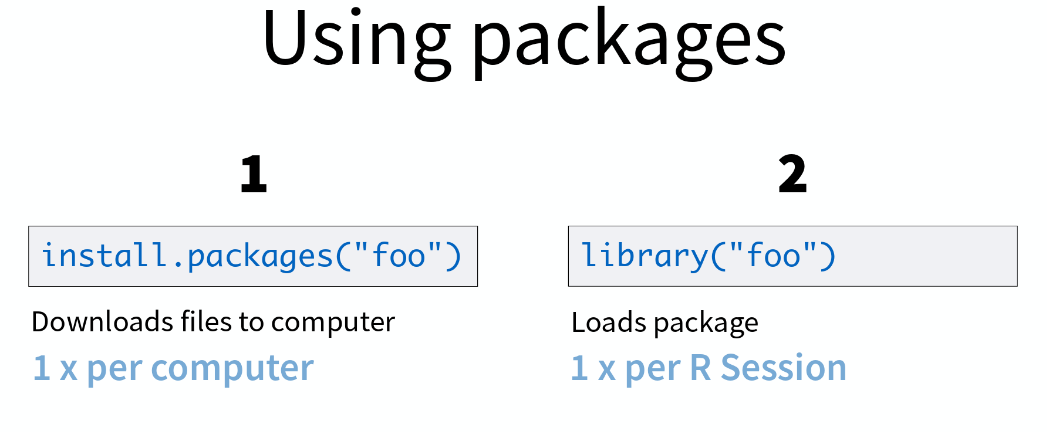
\includegraphics[width=0.9\linewidth]{images/using-packages} \end{center}

\hypertarget{view-and-change-your-working-directory}{%
\subsection{View and Change Your Working
Directory}\label{view-and-change-your-working-directory}}

The working directory is where R pulls files to work with. This is where
your datasets, scripts, etc. live. It can be any folder location. (It
doesn't have to be the same folder where you installed R.)

R always has a working directory set. Get your working directory with
this command in the console: \texttt{getwd()}. You can then set the
working directory in the console using \texttt{setwd()} (must insert
appropriate file path: e.g.~``\textasciitilde/Desktop/''). Verify that
you have the right directory by using \texttt{getwd()} again. Note that
you can see the working directory listed at the top of the Console.

You can also set the working directory via point-and-click:
\texttt{Session} (at the top)--\textgreater{}
\texttt{Set\ Working\ Directory}--\textgreater{}
\texttt{Choose\ Directory}

\hypertarget{to-get-your-file-path}{%
\subsubsection{To get your file path:}\label{to-get-your-file-path}}

\begin{itemize}
\tightlist
\item
  \textbf{Windows users}: Open File Explorer, navigate to the folder you
  want to use, and copy the path at the top of the window. Windows users
  note: the default for Windows is the \texttt{\textbackslash{}}
  (backslash) to separate folders in file paths, but R requires
  \texttt{/} (forward-slash).
\item
  \textbf{Mac users}: Using Finder, navigate to the folder you want to
  use, right click on the folder, and select ``Copy Path.''
\end{itemize}


\end{document}
